\chapter{Simulazione e analisi dei risultati}
\label{chapter:simulation}

In questo capitolo vedremo i risultati delle simulazioni eseguite sul nostro modello. Introdurremo una misura che ci aiuterà a disegnare dei grafici per mettere a confronto simulazioni fatte con strategie di scelta della coda diverse e anche con parametri diversi.

\vspace*{1\baselineskip}

Al fine di analizzare i risultati è stata introdotta la definizione di densità di clienti per ogni step di simulazione; questa misura ci permette di misurare l'affluenza dei clienti nel supermercato e come questa viene gestita dalle casse che hanno il potere di attivarsi o disattivarsi in base alla quantità di clienti presenti. La densità ci permetterà di disegnare i grafici fondamentali che mostrano per ogni simulazione come le casse smaltiscono l'afflusso di clienti in entrata, soprattutto nei periodi critici (in cui il supermercato raggiunge una quantità di clienti che "mettono alla prova" le casse).

La \textbf{densità} di clienti per step corrisponde al numero di clienti medio per ogni cassa; la densità allo step $i$ è:
\begin{equation}
	\text{density}_i = \frac{\# \text{ customers in the supermarket}}{\# \text{ cashdesks}}
\end{equation}
Si terrà conto della densità totale, della densità per le casse standard o self-service e della densità per le casse self-scan.

\section{Simulazione con scopo di validazione}

\paragraph{Stato dell'arte}

Al fine di validare il modello, come primo esperimento è stata condotta una simulazione con gli stessi parametri usati nell'articolo \cite{article1}. Nella loro simulazione il supermercato contiene 20 casse standard e 6 casse self-service; si noti che nel lavoro citato, le casse si attivano o disattivano in base ai dati raccolti dai ricercatori nei supermercati, nel nostro modello invece le casse si attivano in base al numero di clienti presenti nel supermercato, in base a un parametro che è possibile cambiare nel momento in cui si raccolgono i dati. Vengono messe a confronto le strategie diverse di scelta della coda da parte dei clienti, arrivando alla conclusione che la strategia che porta al minor tempo d'attesa è quella chiamata "minimo tempo d'attesa in base alla \textit{power regression}" nel capitolo \ref{implementation:intro}; tuttavia i risultati portano a dire che questo scenario non è quello ottimale per tutti i supermercati negli orari di punta.

Nelle prossime simulazioni verrà testato il jockeying, in particolare si metteranno a confronto le diverse strategie di scelta della coda e di jockeying per stabilire se questo porti a un miglioramento dell'esperienza del cliente nel supermercato. Questi esperimenti verranno poi messi a confronto con una simulazione in cui c'è soltanto la coda condivisa per le casse standard, pertanto i clienti non avranno bisogno di scegliere la coda nè di fare jockeying: in base a quanto detto nell'articolo \cite{yanagisawa2011methods}, questo tipo di coda dovrebbe portare a tempi di attesa minori. 
Verranno quindi introdotte nella simulazione le casse self-scan con rilettura randomica, si prevede che queste portino a una diminuzione considerevole dei tempi d'attesa in coda, in quanto viene a mancare la fase di scanner da parte dei cassieri. Infine verrà effettuata una simulazione con gli elementi probabilistici già descritti nel corso dei capitoli \ref{chapter:model} e \ref{implementation:intro}, che rendono l'esperimento non deterministico e a nostro riguardo più realistico.

\paragraph{Simulazione con gli stessi parametri}

Come validazione sono state effettuate delle simulazioni con gli stessi parametri usati nell'articolo \cite{article1}: 20 casse standard con code parallele, 6 casse self-service, no jockeying; è stata ripetuta la stessa simulazione 4 volte però con le 4 strategie diverse di scelta della coda.

\begin{figure}[H]
	\centering
	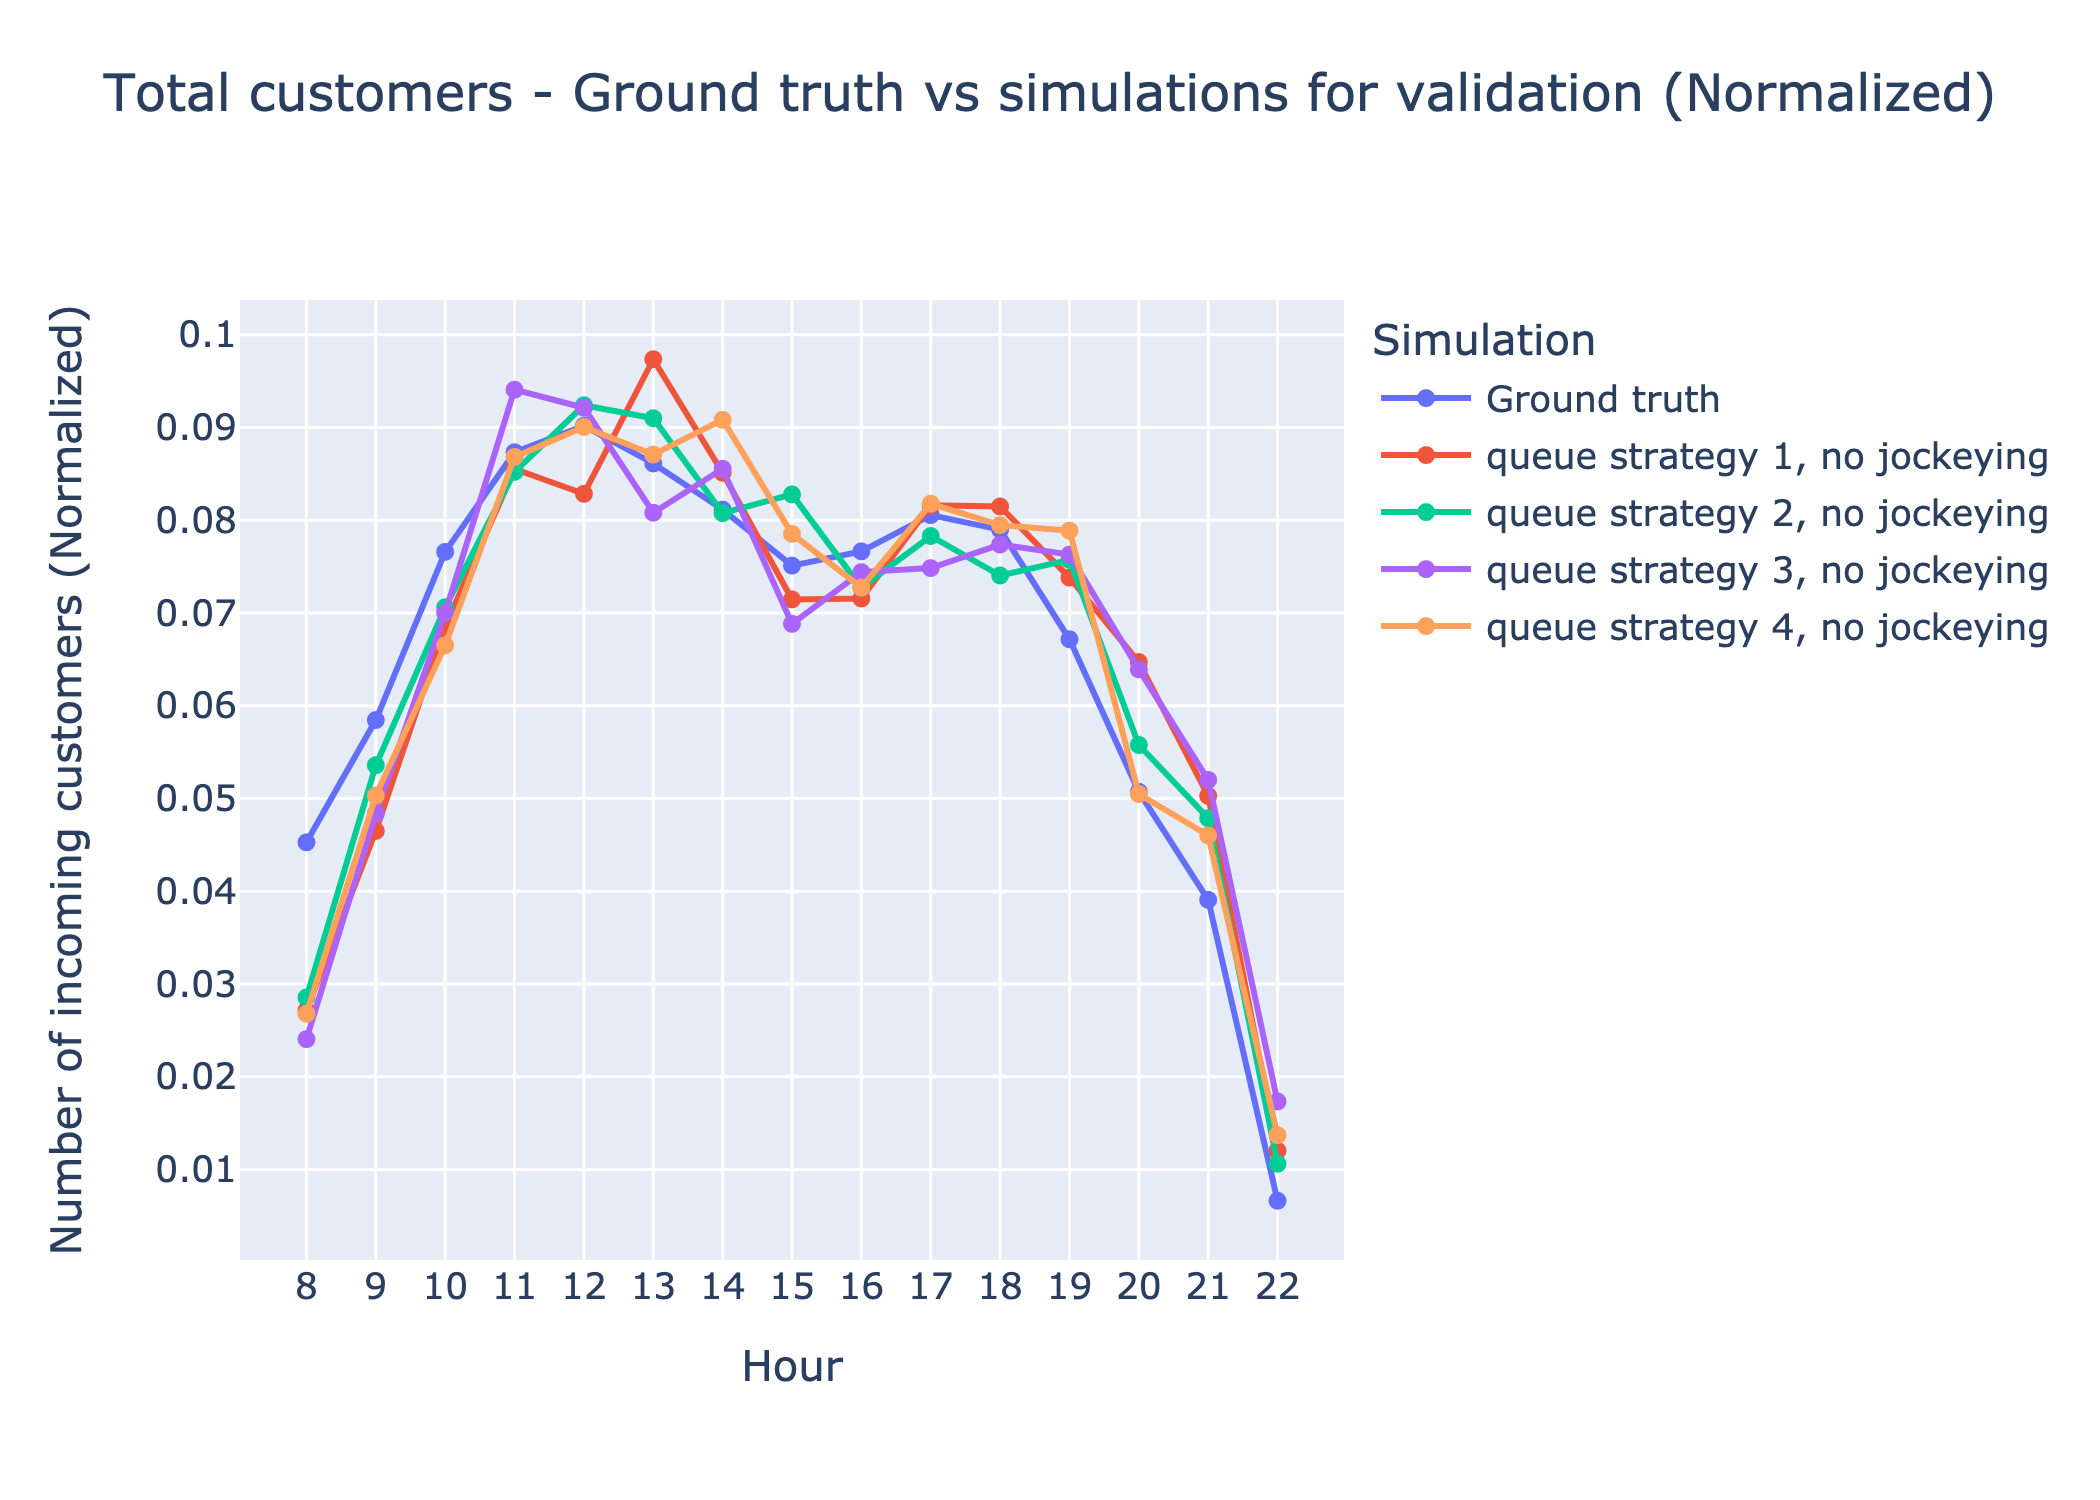
\includegraphics[width=12cm]{"images/results/total_customers_validation.png"}
	\label{fig:total_customers_validation}
	\caption{Numero di clienti totali al variare dell'ora}
\end{figure}

Il grafico \ref{fig:total_customers_validation} funge da validazione: mettiamo a confronto il numero totale di clienti (normalizzati) presenti nel negozio ad ogni ora per ogni simulazione e per la simulazione dell'articolo. Si nota come, a parità di parametri, il nostro modello e il modello di \cite{article1} sopportino allo stesso modo il numero di clienti presenti nel negozio, facendoli defluire in modo paragonabile.

\begin{figure}[H]
	\centering
	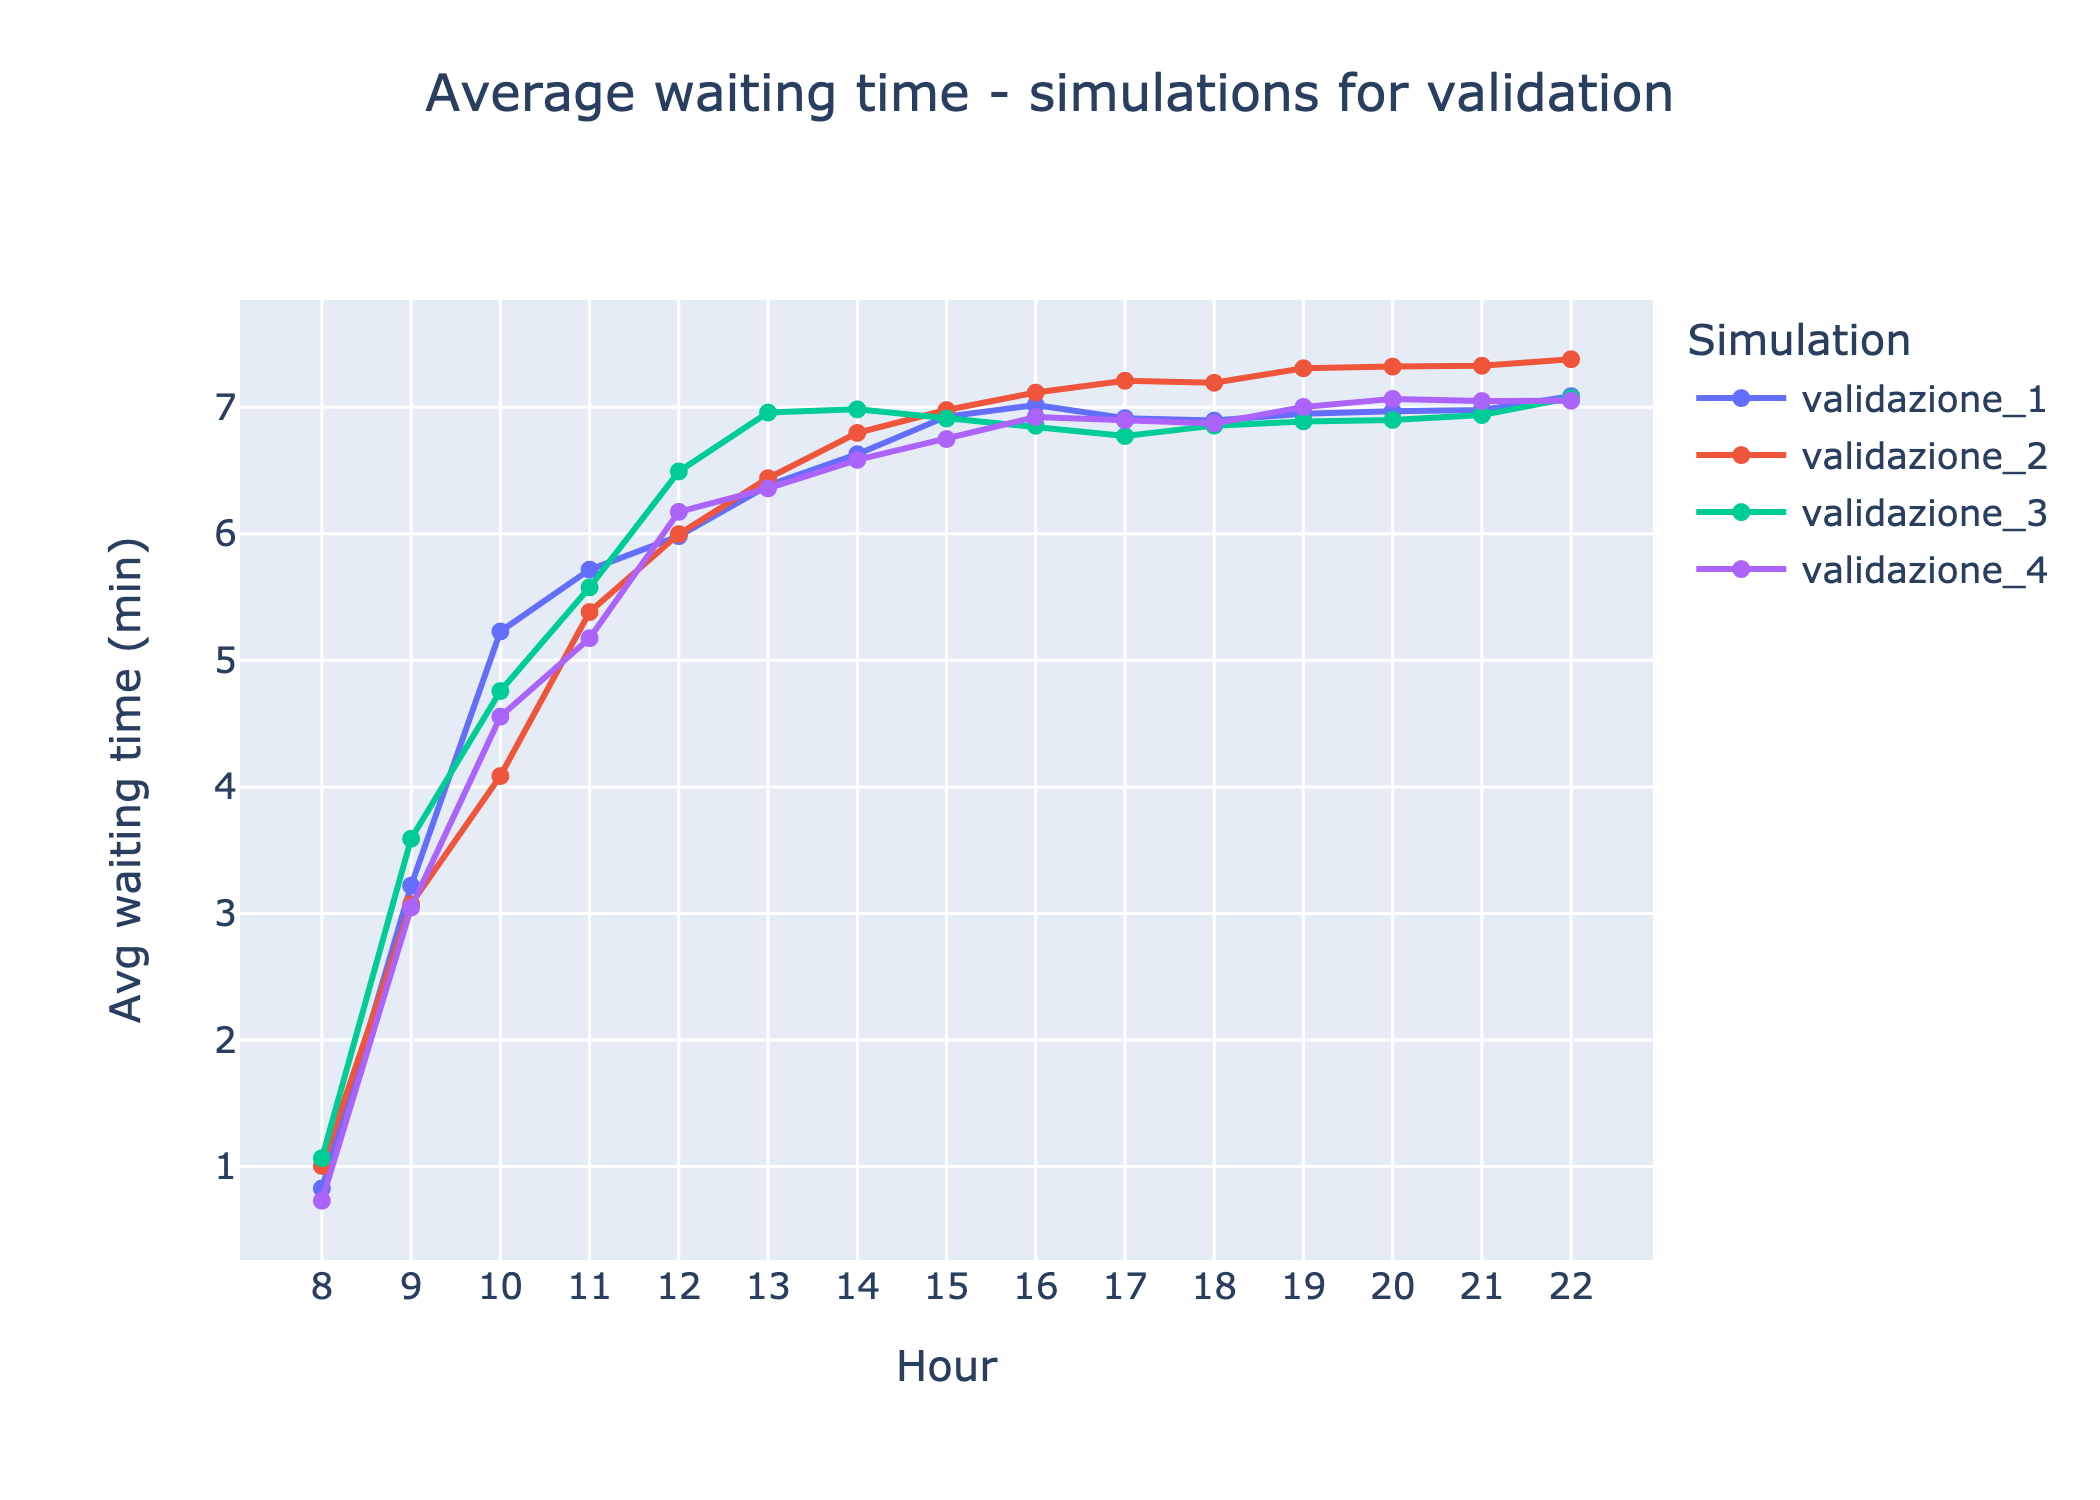
\includegraphics[width=12cm]{"images/results/avg_wt_validation.png"}
	\label{fig:avg_wt_validation}
	\caption{Tempo medio d'attesa al variare dell'ora}
\end{figure}


Nell'immagine \ref{fig:avg_wt_validation} si può vedere la variazione del tempo medio di attesa in coda dei clienti nel corso della giornata lavorativa che va dalle 8:00 alle 22:00. Le simulazioni variano per strategia di scelta della coda da parte dei clienti, si nota quindi che, in assenza di jockeying, la strategia 3 risulta quella che durante l'arco della giornata mantiene il tempo medio più basso, anche se a fine giornata tutte e 4 le strategie raggiungono una media paragonabile.

Nelle prossime simulazioni verranno aggiunte delle caratteristiche che pensiamo possano migliorare il tempo medio d'attesa dei clienti, che metteremo a confronto con questa simulazione la quale rappresenta il nostro punto di partenza.

\section{Simulazione con strategie \textit{jockey}}

Introduciamo dunque le 2 strategie di jockey descritte nel capitolo \ref{implementation:intro}. In queste simulazioni sono presenti 20 casse normali con code parallele, 6 casse self-service, 4 strategie di scelta della coda e 2 strategie di jockeying, per un totale di 8 simulazioni.

\begin{figure}[H]
	\centering
	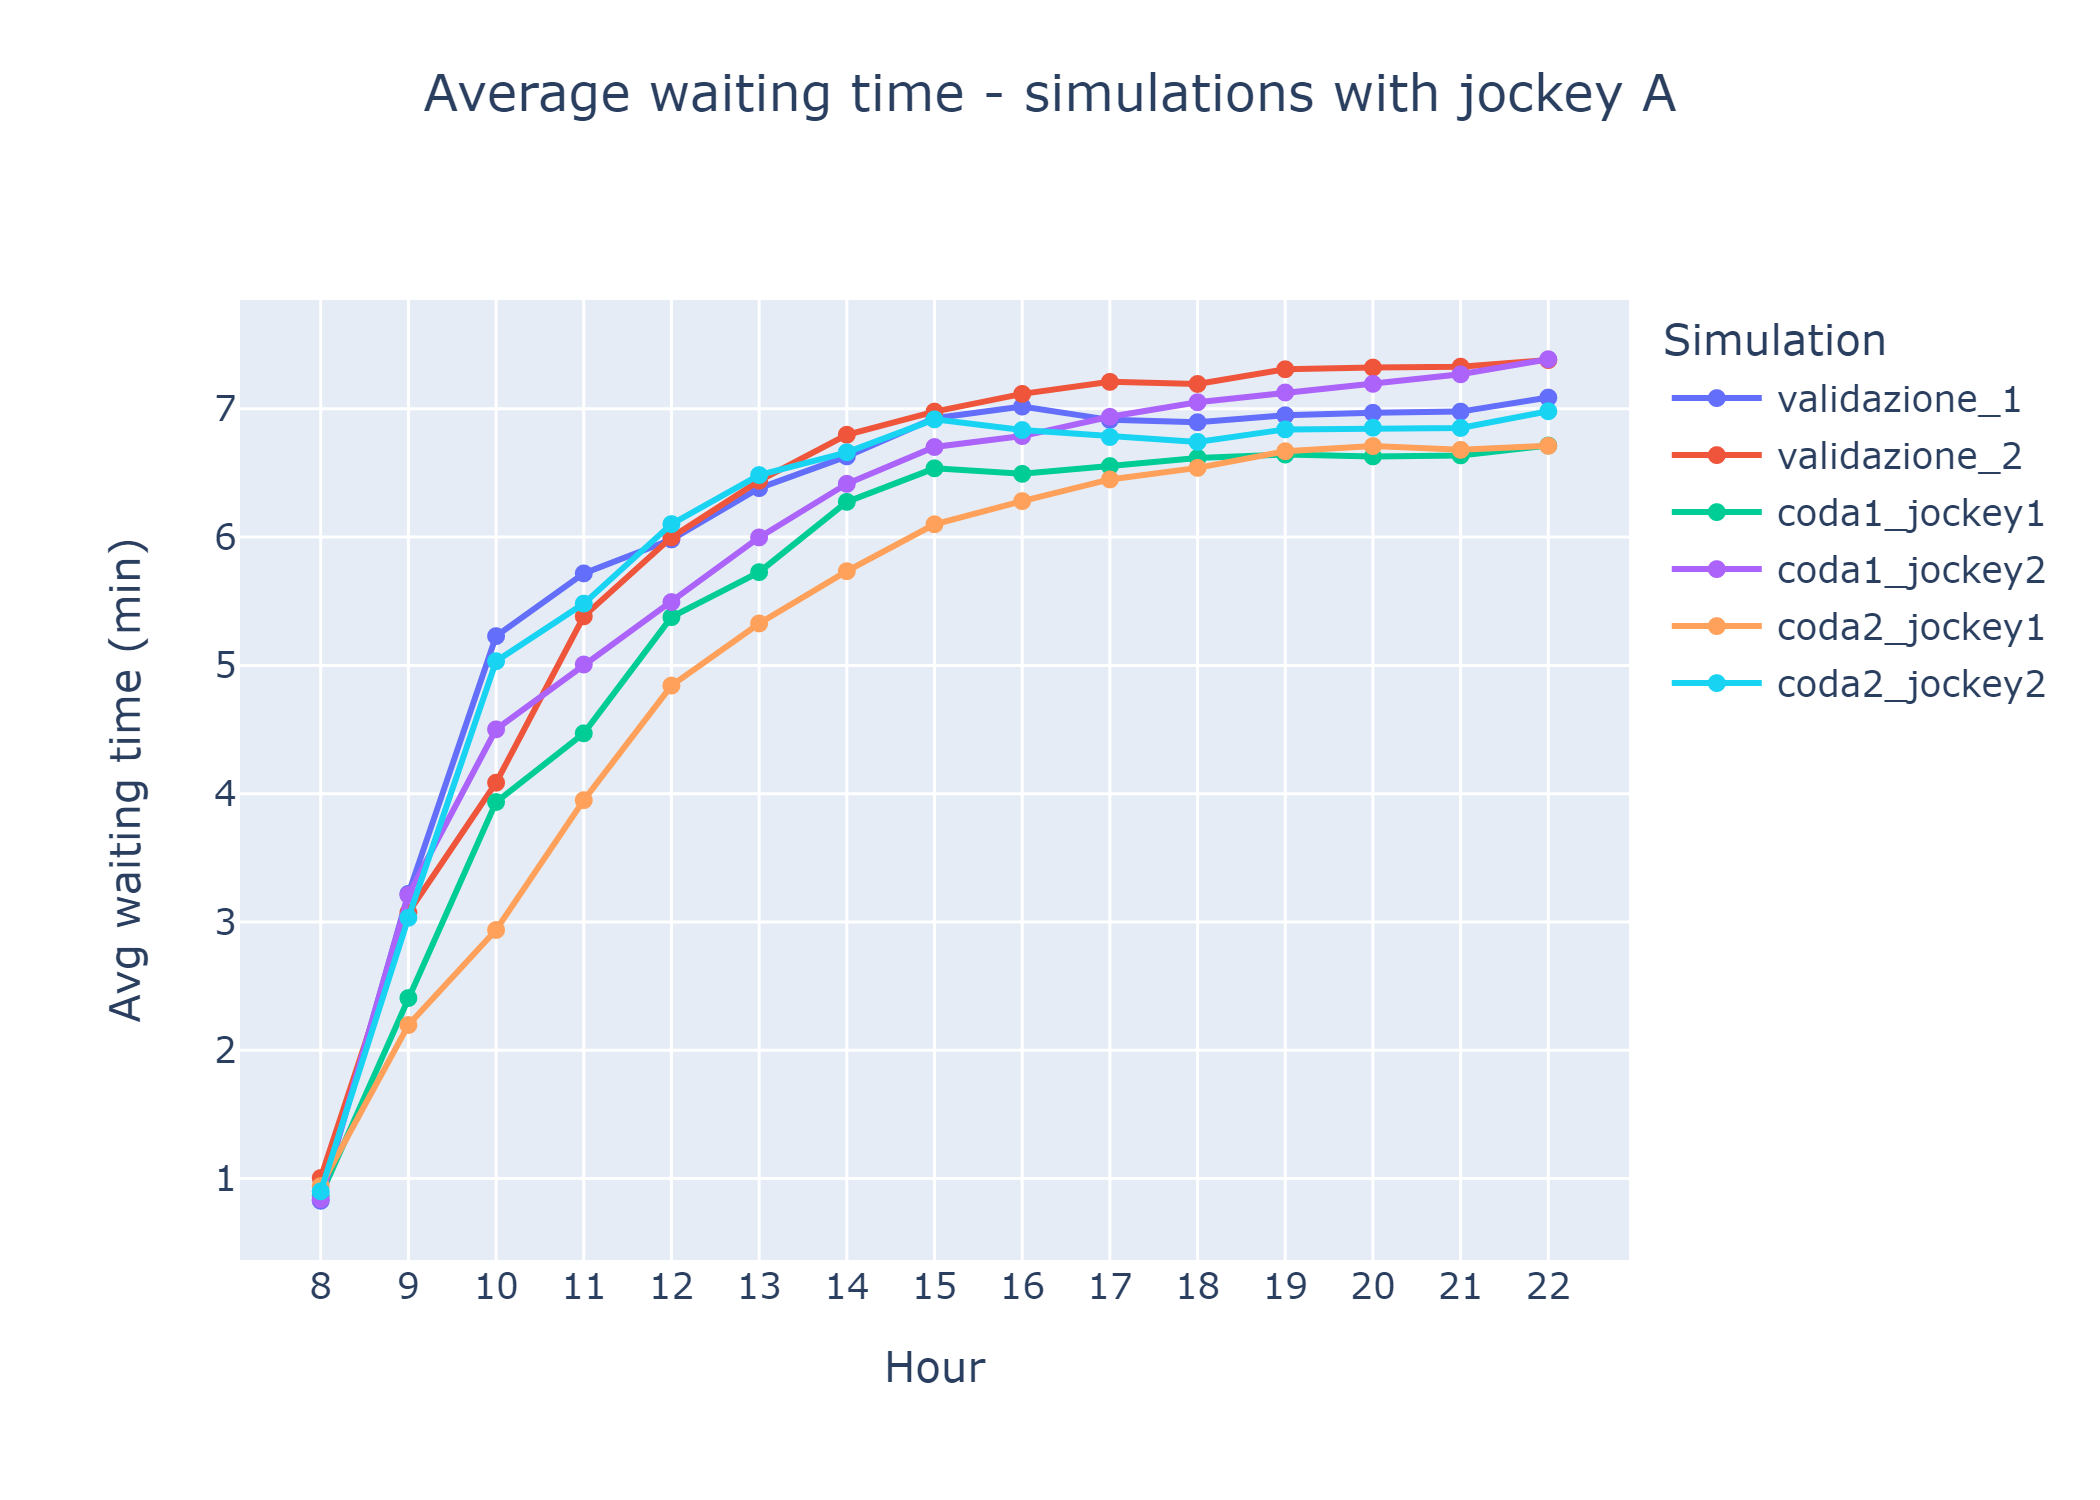
\includegraphics[width=12cm]{"images/results/avg_wt_jockey_a.png"}
	\label{fig:avg_wt_jockey_a}
	\caption{Tempo medio d'attesa al variare dell'ora}
\end{figure}

Nell'immagine \ref{fig:avg_wt_jockey_a} si mettono a confronto 2 strategie di scelta della coda: minimo numero di elementi, minimo numero di persone in coda. Le due strategie sono affiancate da nessun jockeying, jockey per minimo numero di elementi e jockey per minimo numero di persone in coda. \\ 
Si osserva che i risultati migliori si raggiungono quando si fa jockey e inoltre la strategia di scelta della coda è la stessa del jockey, con una diminuzione massima del tempo medio di attesa di circa 2 timestamp (1 minuto) e della media finale di 1 timestamp (30 secondi) rispetto alle simulazioni senza jockey. Si può dire pertanto che mischiare le strategie, ad esempio scegliendo la coda per numero di persone e facendo jockey per numero di elementi nei carrelli, peggiori le prestazioni del sistema rispetto al tempo di attesa dei clienti. Questo è in linea con quanto si osserva nell'articolo \cite{xu1996dynamic}, che afferma	che a parità di parametri un sistema con jockeying è più efficiente di uno senza.

\begin{figure}[H]
	\centering
	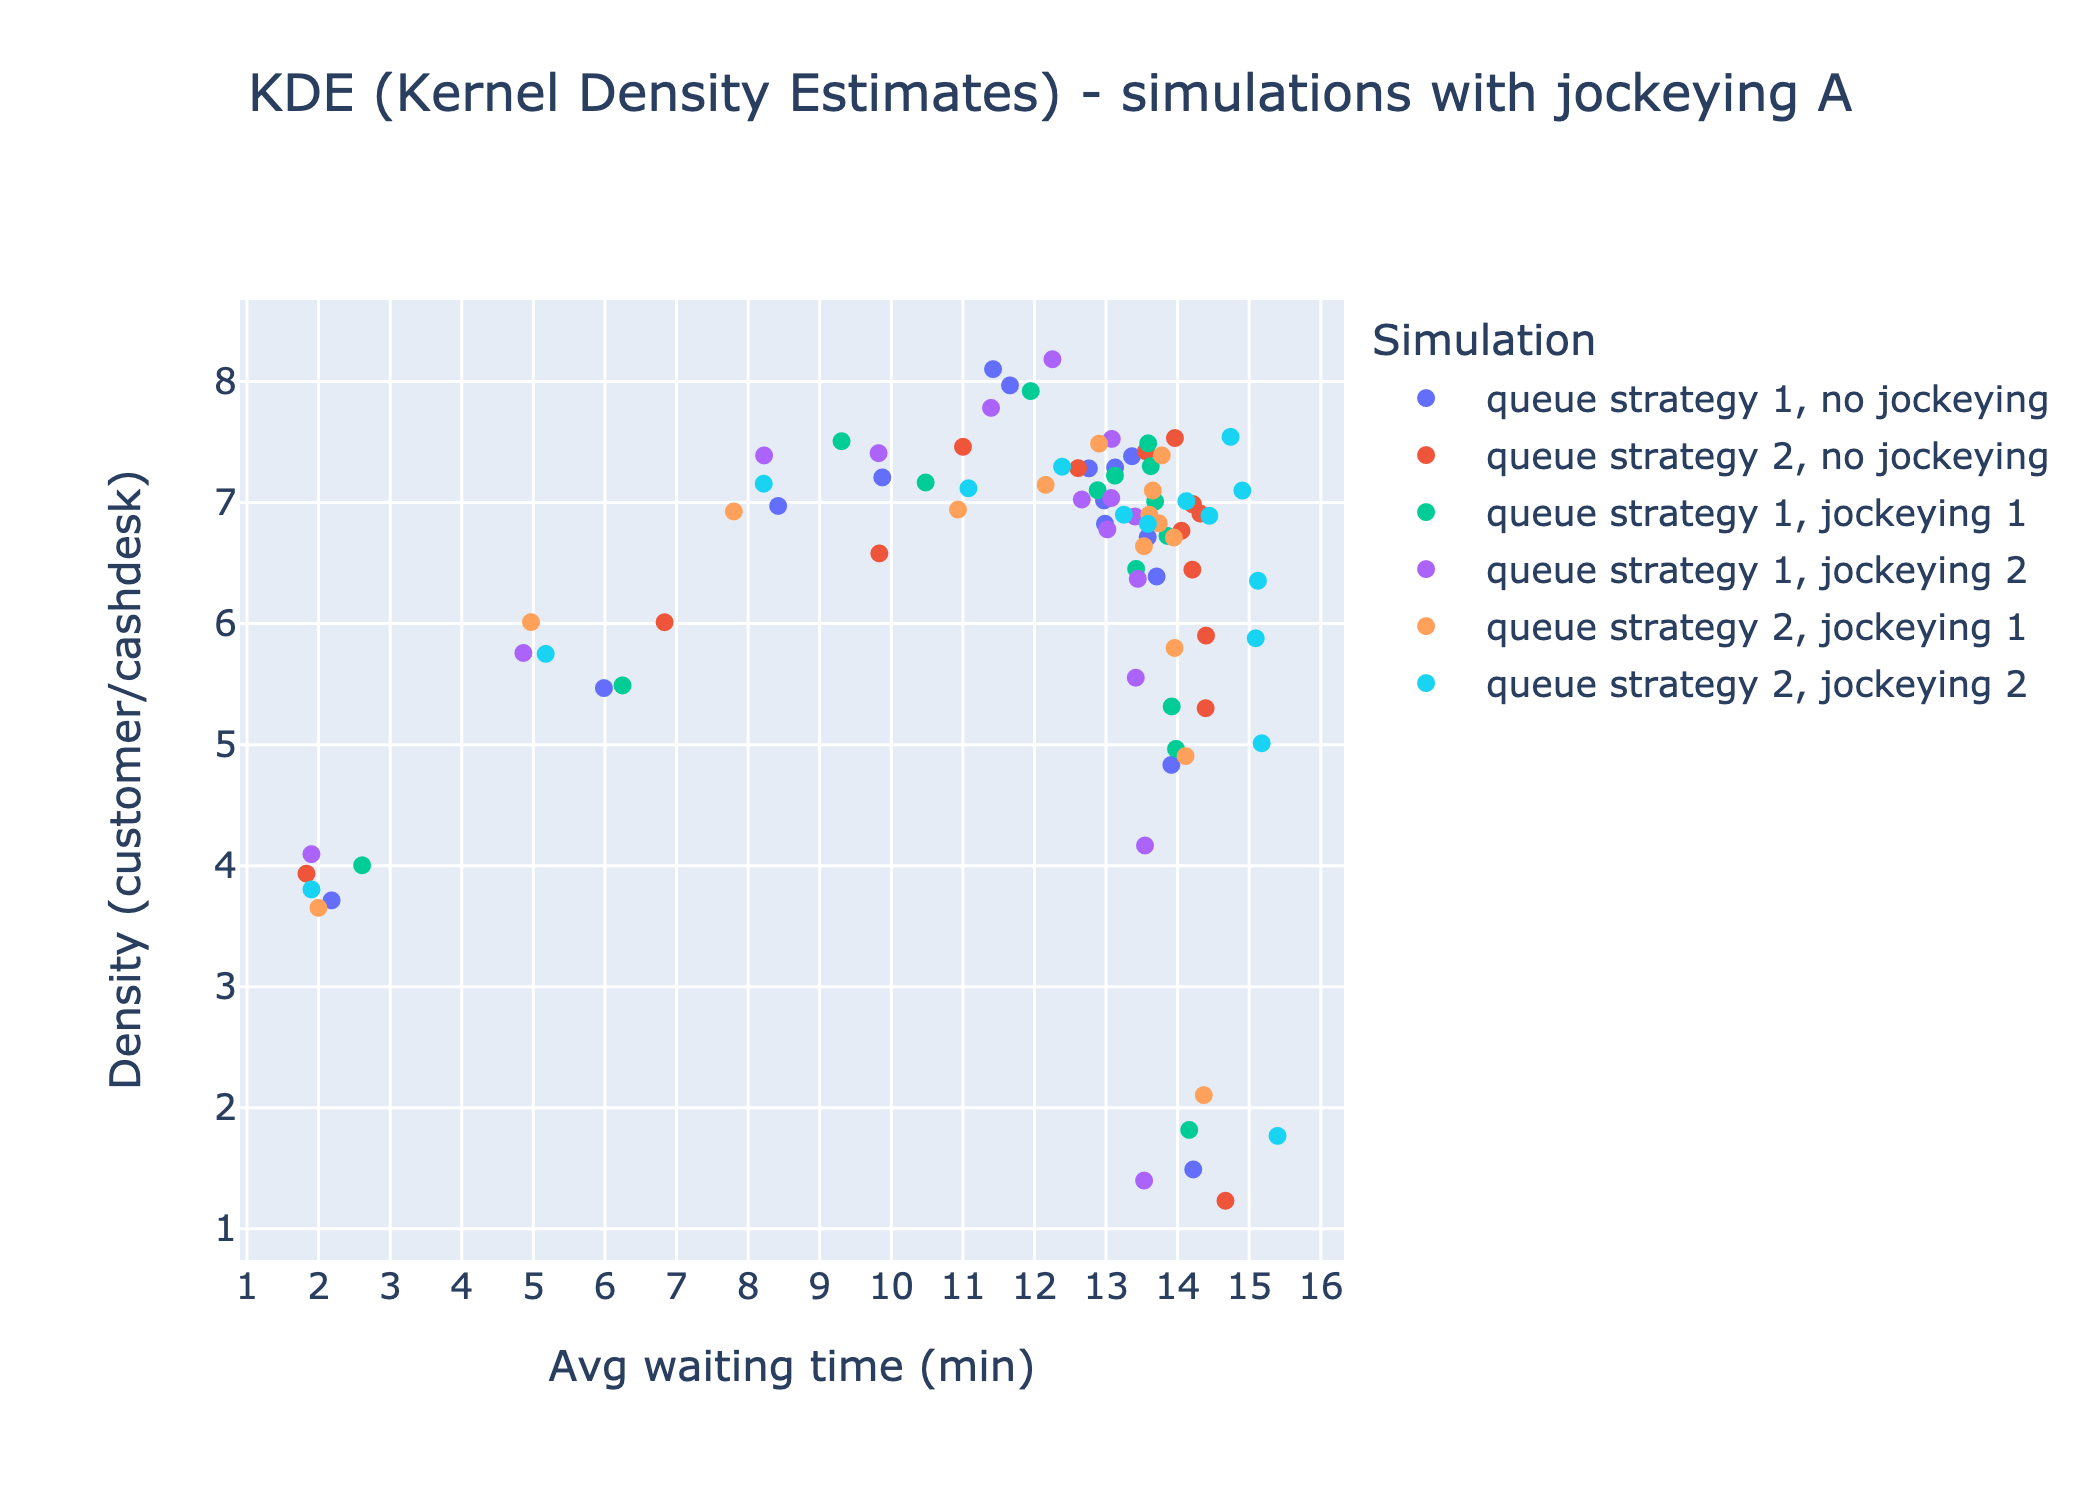
\includegraphics[width=12cm]{"images/results/kde_jockey_a.png"}
	\label{fig:kde_jockey_a}
	\caption{KDE - densità al variare del tempo medio d'attesa}
\end{figure}

Nell'immagine \ref{fig:kde_jockey_a} è riportato un grafico KDE (Kernel Density Estimates), che mostra la densità di clienti nel negozio (come definita a inizio capitolo) al variare del tempo medio d'attesa. Questo grafico mostra che con l'aumentare della quantità di clienti nel negozio aumenta anche il tempo d'attesa in coda, come ci si aspetterebbe; si nota che viene raggiunto un "punto critico" in cui sia la densità che il tempo medio d'attesa sono molto alti, superato il quale il sistema reagisce facendo defluire più rapidamente i clienti, il cui tempo d'attesa medio crolla. Questo accade sia perchè le casse vengono aperte dato che il numero di clienti aumenta e anche perchè raggiunta una certa ora il negozio chiude e non entrano più clienti.

\begin{figure}[H]
	\centering
	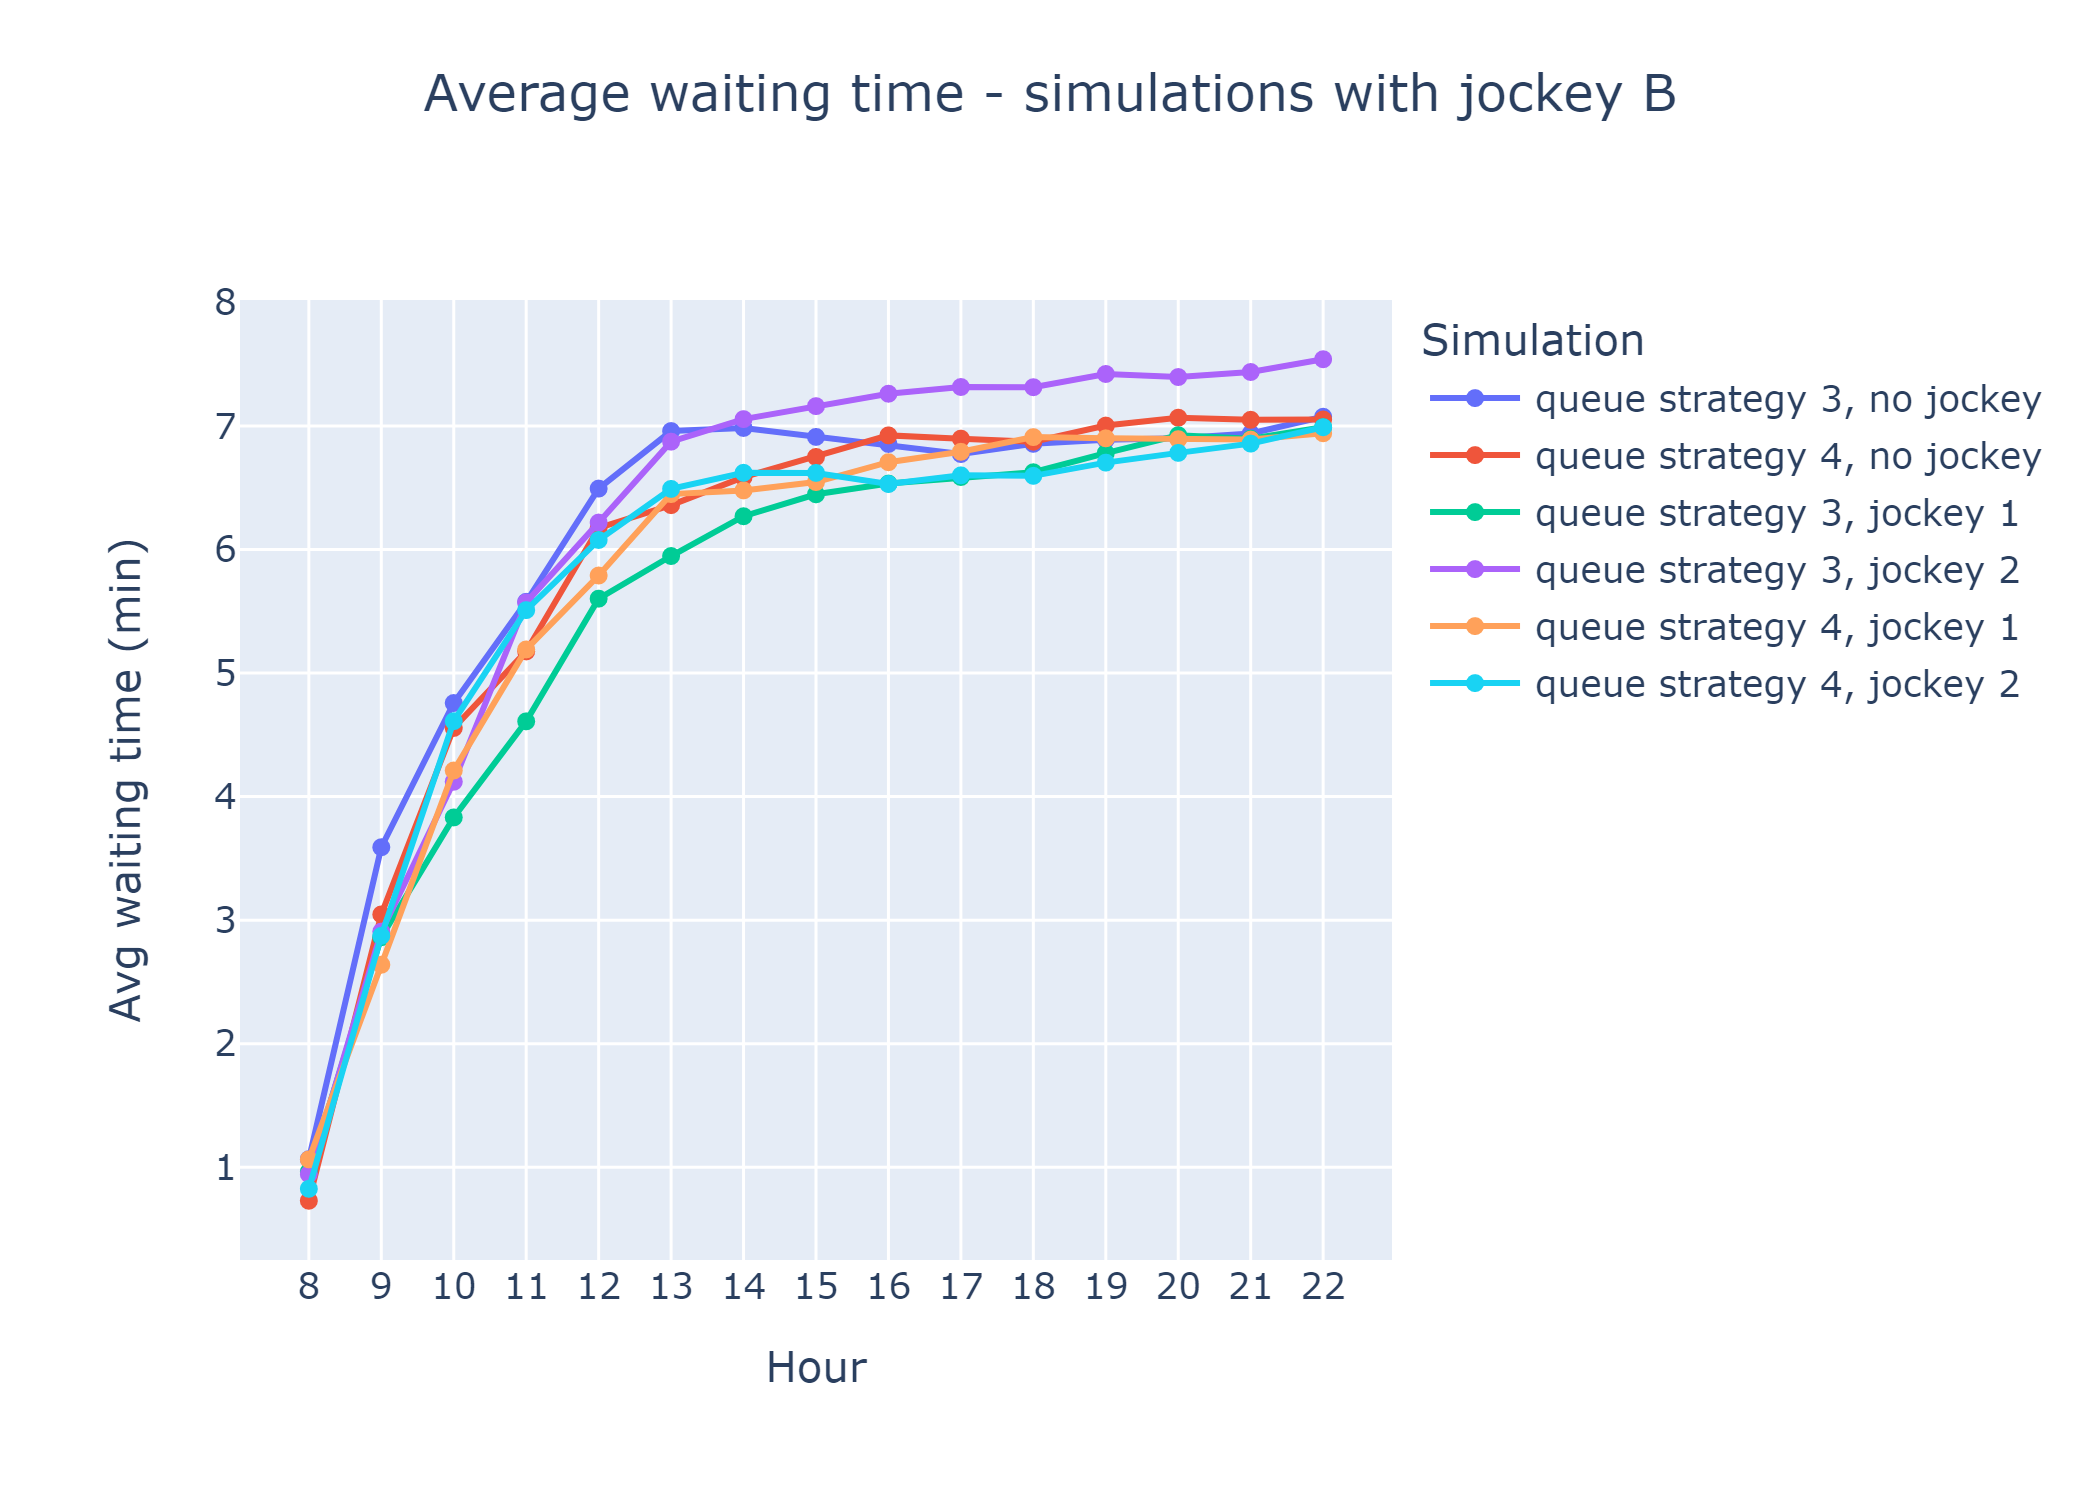
\includegraphics[width=12cm]{"images/results/avg_wt_jockey_b.png"}
	\label{fig:avg_wt_jockey_b}
	\caption{Tempo medio d'attesa al variare dell'ora}
\end{figure}

Nell'immagine \ref{fig:avg_wt_jockey_b} vengono messe a confronto 2 strategie di scelta della coda: minimo tempo d'attesa in base al tempo di servizio medio, minimo tempo d'attesa in base alla power regression. Le due strategie sono affiancate da nessun jockeying, jockey per minimo numero di elementi e jockey per minimo numero di persone in coda. \\
In questo caso non vale quanto detto sopra, le strategie di scelta della coda e di jockey non possono essere le stesse e non si può dire che affiancandole si ottengono risultati migliori; questo potrebbe rappresentare un ulteriore studio da fare per allargare il nostro modello.

Si nota come la strategia di scelta della coda che mantiene il tempo d'attesa medio minore durante tutta la giornata sia la power regression affiancata da jockey per minimo numero di persone in coda; questa simulazione raggiunge un tempo medio d'attesa minore finale di circa 1.5 timestamp rispetto alla simulazione peggiore. Questa però è comunque molto vicina al tempo medio della strategia di scelta della coda per minimo tempo di servizio medio e senza jockeying, anche se quest'ultima tende a peggiorare nell'ora finale.

\begin{figure}[H]
	\centering
	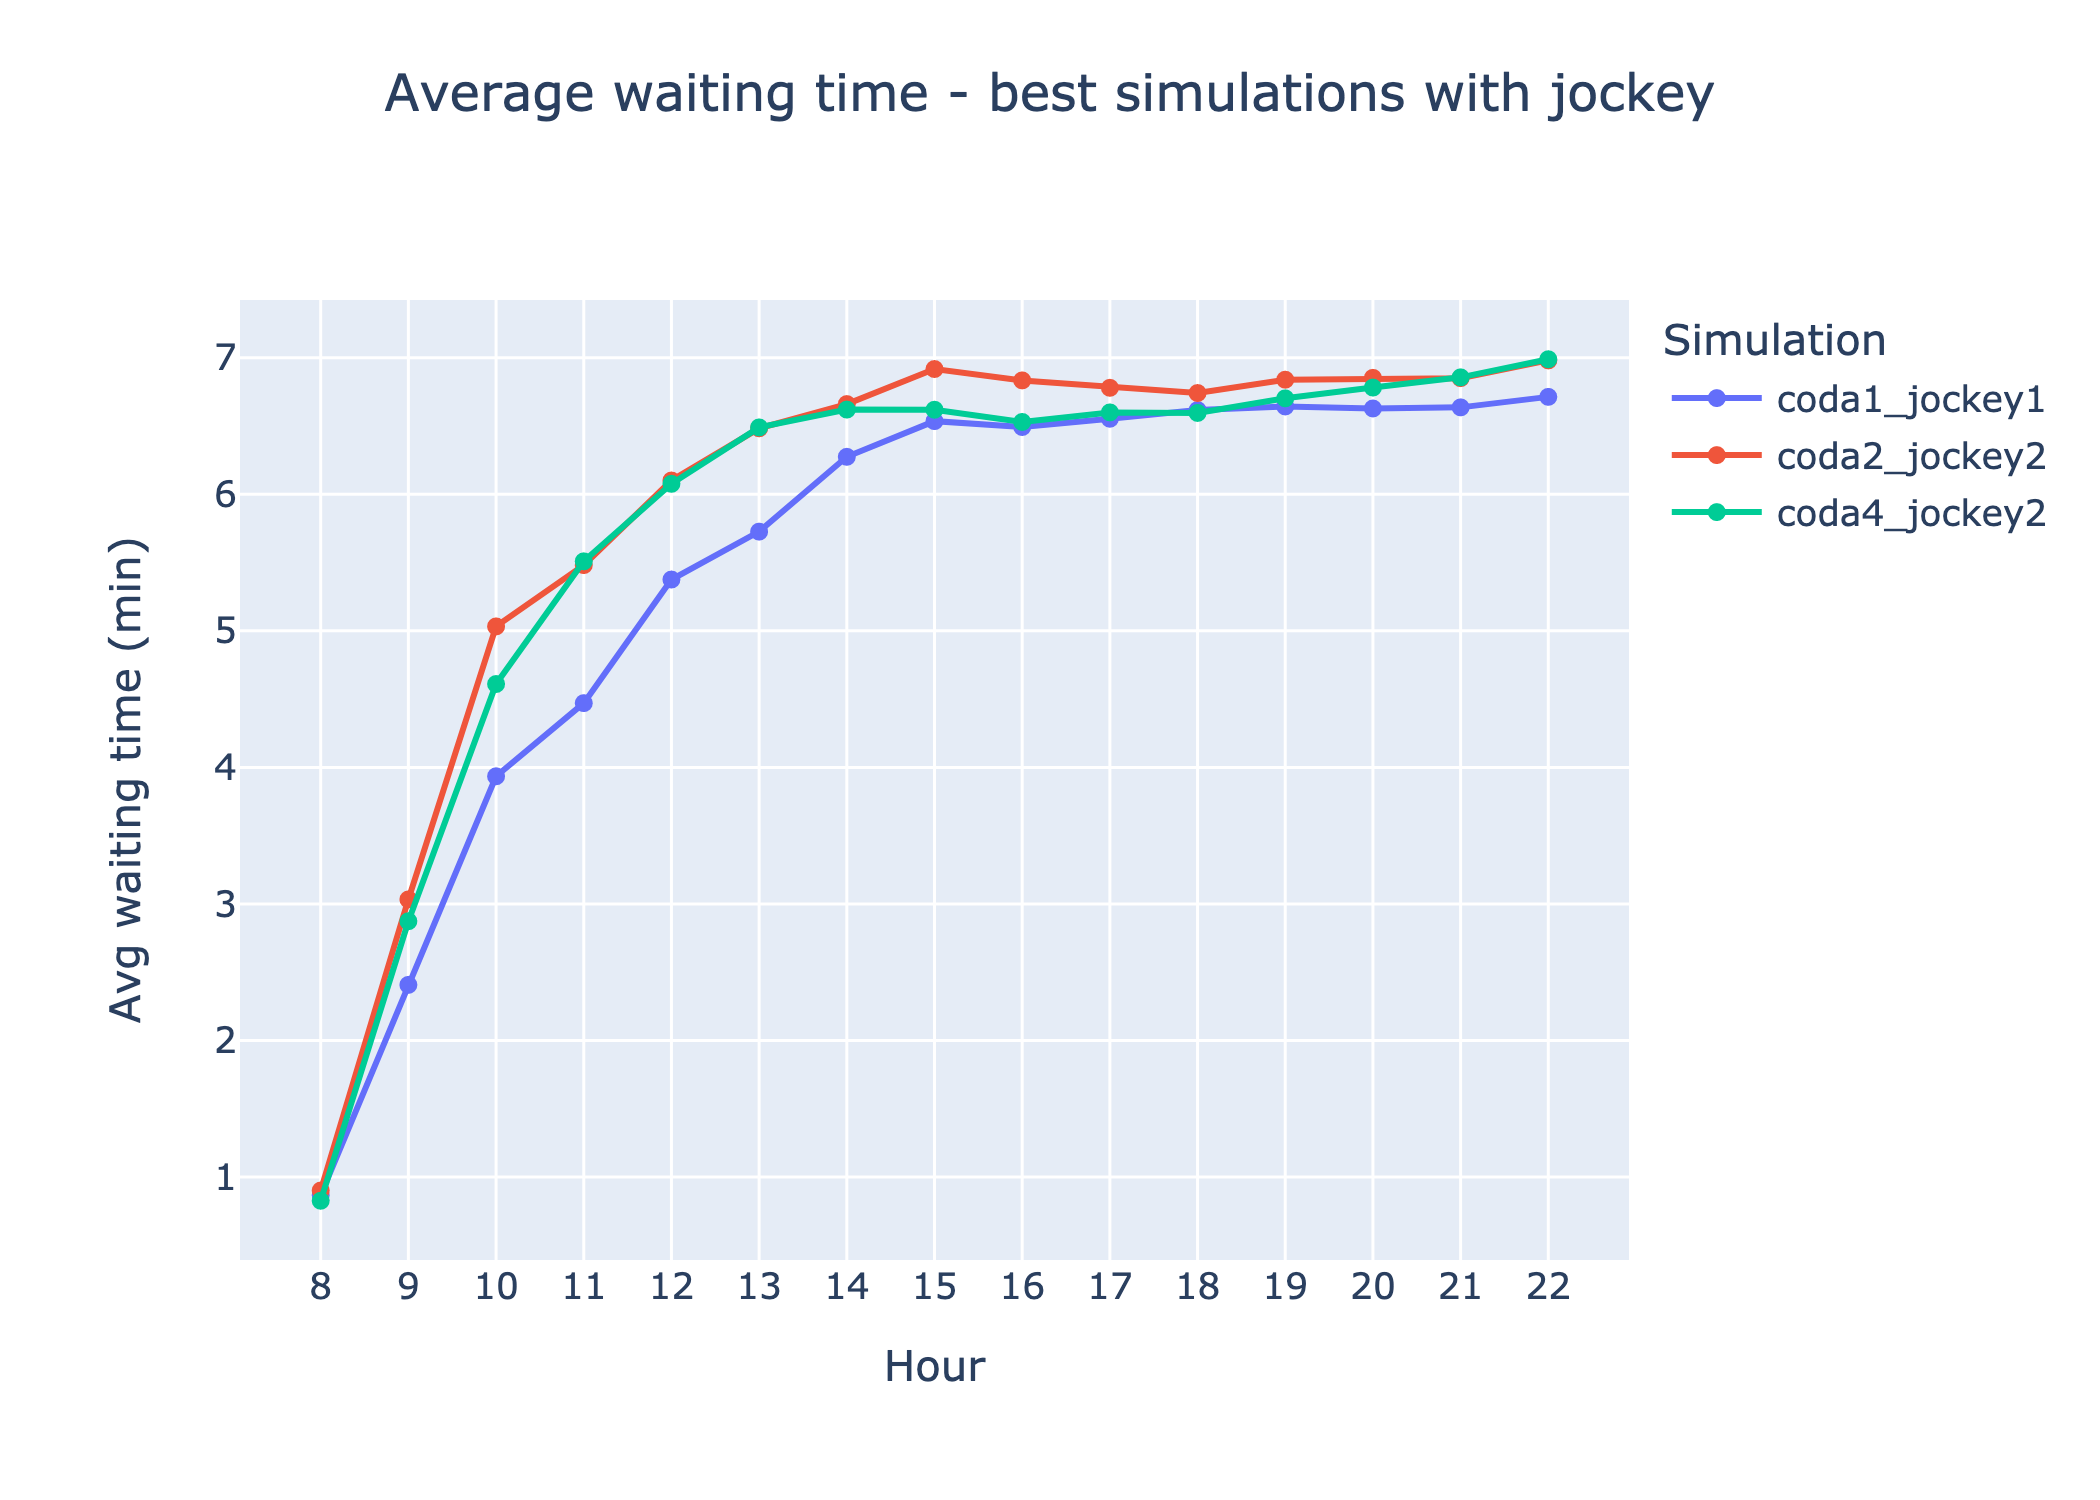
\includegraphics[width=12cm]{"images/results/avg_wt_jockey_best.png"}
	\label{fig:avg_wt_jockey_best}
	\caption{Tempo medio d'attesa al variare dell'ora}
\end{figure}

Nel grafico \ref{fig:avg_wt_jockey_best} mettiamo a confronto il tempo medio d'attesa delle migliori strategie viste fin ora: il tempo medio finale è circa lo stesso per tutte e tre, ma si nota che il grafico della prima strategia rimane sotto gli altri nell'arco di tutta la giornata.

\section{Simulazione con coda condivisa}

Con le prossime simulazioni indagheremo sulla diminuzione del tempo medio d'attesa nel caso di coda condivisa (N-fork): metteremo a confronto la strategia migliore trovata fin ora (scelta della coda e jockey per minimo numero di elementi) con il caso di una coda condivisa per tutte le casse. \\
Come già specificato, nei casi esaminati fin ora le casse si aprivano e chiudevano in maniera automatica in base al numero di clienti presenti nel negozio e che necessitano di essere serviti; nel caso di coda condivisa questa funzione non è stata implementata, e potrebbe rappresentare un'estensione del nostro modello. Per questo motivo abbiamo deciso di diminuire il numero di casse nella simulazione: in base a osservazioni fatte in fase sperimentale abbiamo notato che il numero di casse aperte massimo in un dato momento è 8, chiaramente rispetto alla distribuzione dei clienti in entrata utilizzata; per questo motivo abbiamo voluto indagare i casi di 5, 6, 7 e 8 casse standard presenti nel negozio (e 6 casse self-service come fatto in precedenza).

\begin{figure}[H]
	\centering
	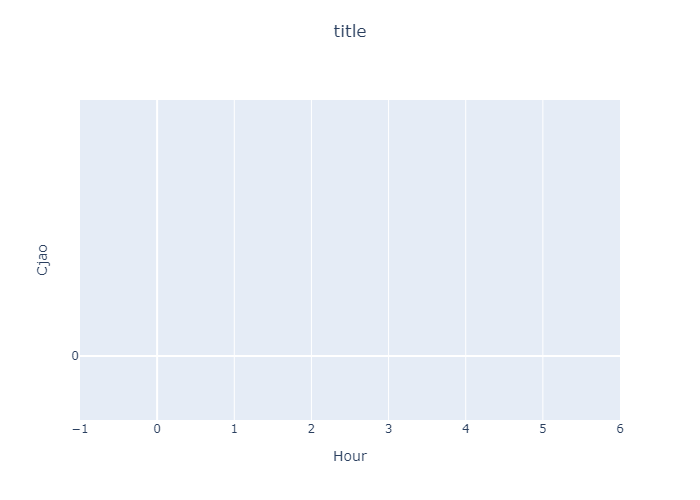
\includegraphics[width=12cm]{"images/results/avg_wt_codacondivisa.png"}
	\label{fig:avg_wt_codacondivisa}
	\caption{Tempo medio d'attesa al variare dell'ora}
\end{figure}

Nel grafico \ref{fig:avg_wt_codacondivisa} riportiamo i tempi medi d'attesa delle simulazioni con code parallele e jockey rappresentandoli con delle linee, e i tempi medi d'attesa delle simulazioni con coda condivisa rappresentandoli con dei trattini. Si nota immediatamente che nel caso di 5 casse il tempo medio d'attesa sale vertiginosamente a circa 20 minuti sia per le code parallele che per la coda condivisa: questo è imputabile alla distribuzione dei clienti in entrata, il supermercato con 5 casse è troppo piccolo per gestire questa quantità. \\
Una cosa interessante da notare invece è la divisione netta nel grafico tra le simulazioni con code parallele e quelle con coda condivisa: l'utilizzo della coda condivisa abbassa i tempi medi d'attesa durante tutta la giornata, anche rispetto al caso in cui i clienti fanno jockey. Questi risultati sono in linea con l'articolo \cite{yanagisawa2011methods}, in cui si mette in luce il fatto che l'utilizzo di una coda condivisa migliori le prestazioni del negozio.

\begin{figure}[H]
	\centering
	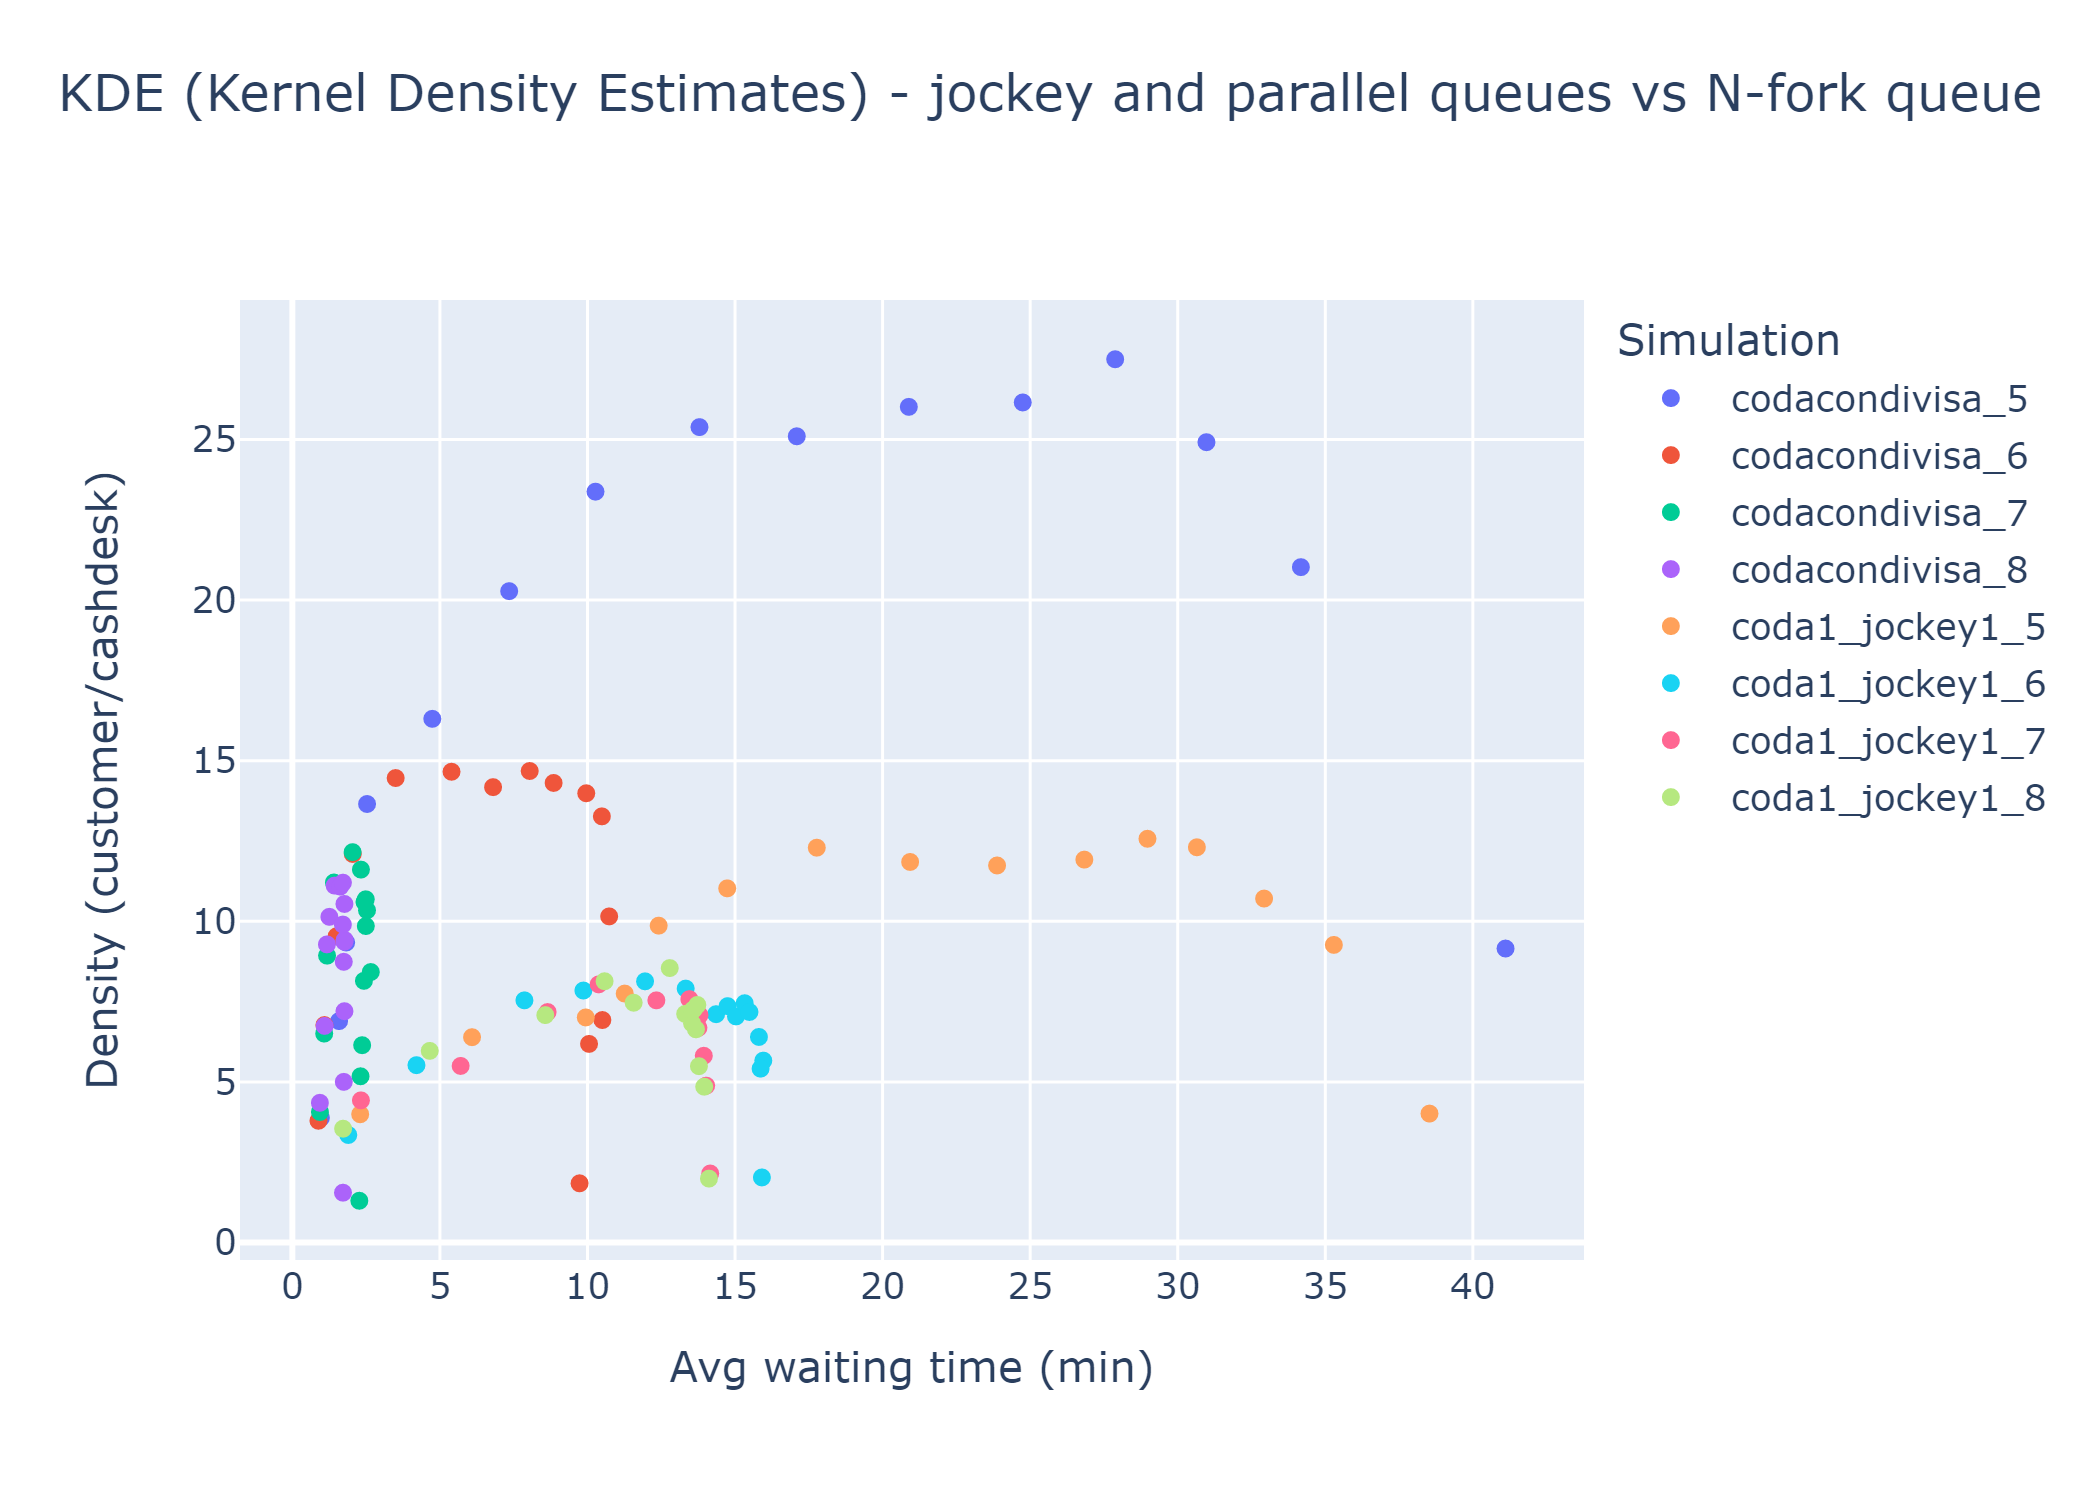
\includegraphics[width=12cm]{"images/results/kde_codacondivisa.png"}
	\label{fig:kde_codacondivisa}
	\caption{KDE - densità al variare del tempo medio d'attesa}
\end{figure}

Nell'immagine \ref{fig:kde_codacondivisa} è riportato il grafico KDE delle stesse simulazioni del grafico precedente. Si nota ancora come il negozio con 5 casse non abbia delle buone prestazioni rispetto alla quantità di clienti entranti, sia nel caso di code parallele che nel caso di coda condivisa. Possiamo osservare però che nel caso delle code condivise si arriva a toccare livelli di densità di clienti più alti, questo accade per un limite del modello, infatti se la coda arriva alla sua capienza massima, i clienti attendono che si liberi per mettersi in coda, creando così più traffico nella zona di shopping, come si può vedere nell'immagine \ref{fig:codacondivisa_screenshot}; dopo aver superato il momento critico, il grafico ci mostra che il sistema che utilizza l'N-fork è in grado di ritornare meglio a livelli di densità minori del sistema con code parallele, il tutto mantenendo un tempo medio d'attesa basso.

\begin{figure}[H]
	\centering
	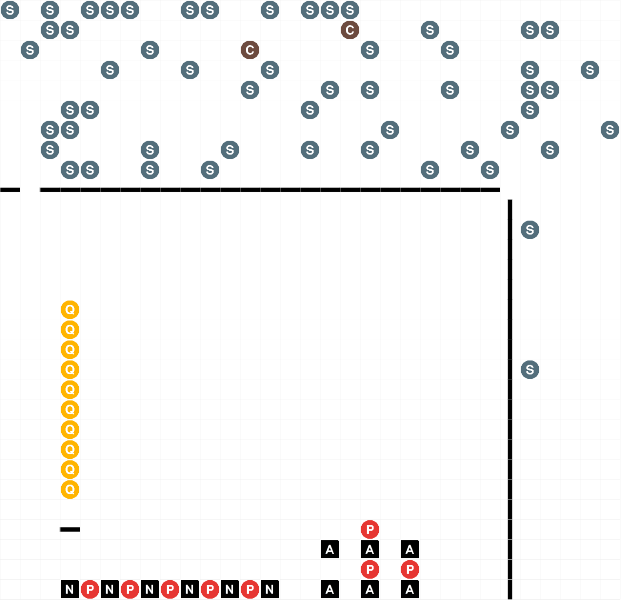
\includegraphics[width=12cm]{"images/results/codacondivisa_screenshot.png"}
	\label{fig:codacondivisa_screenshot}
	\caption{Screenshot della simulazione con coda quasi al limite}
\end{figure}

\section{Simulazione con casse self-scan}

In questa simulazione vedremo il caso in cui nel supermercato sono presenti solamente casse self-scan, in particolare 7; in questa simulazione chiaramente tutti i clienti si recheranno alla cassa self-scan, la probabilità di una rilettura parziale è del $2\%$ e una rilettura totale è dell'$1\%$.

\begin{figure}[H]
	\centering
	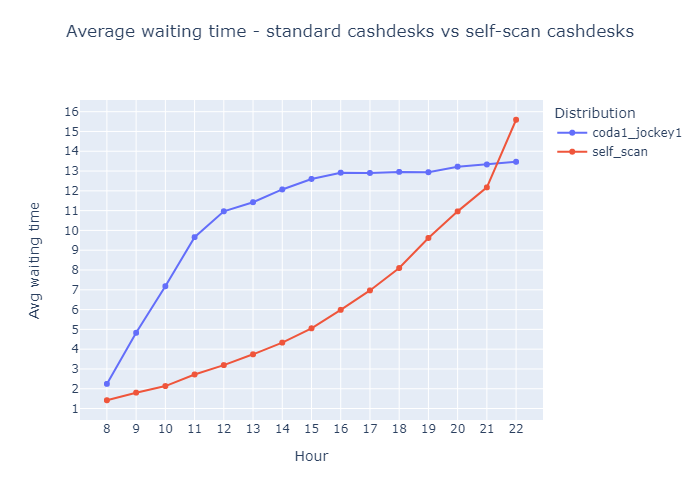
\includegraphics[width=12cm]{"images/results/avg_wt_selfscan.png"}
	\label{fig:avg_wt_selfscan}
	\caption{Tempo medio d'attesa al variare dell'ora}
\end{figure}

Si nota immediatamente dal grafico \ref{fig:avg_wt_selfscan} che il tempo medio d'attesa della simulazione con self-scan va ad aumentare sempre più; questo accade a causa delle riletture, infatti i clienti che non ricevono una rilettura escono immediatamente dal negozio, mentre gli altri restano in coda ad una sola cassa, che funge da collo di bottiglia. Aumentando la probabilità di rilettura, infatti, la simulazione fallisce perchè la coda alla cassa riservata diventa troppo lunga. \\
Rispetto a questa simulazione bisognerebbe avere dati più completi, ad esempio sapere con che probabilità vengono fatte le riletture nei supermercati o con che distribuzione entrano in negozio i clienti self-scan; questa è una possibile estensione del nostro lavoro.

\begin{figure}[H]
	\centering
	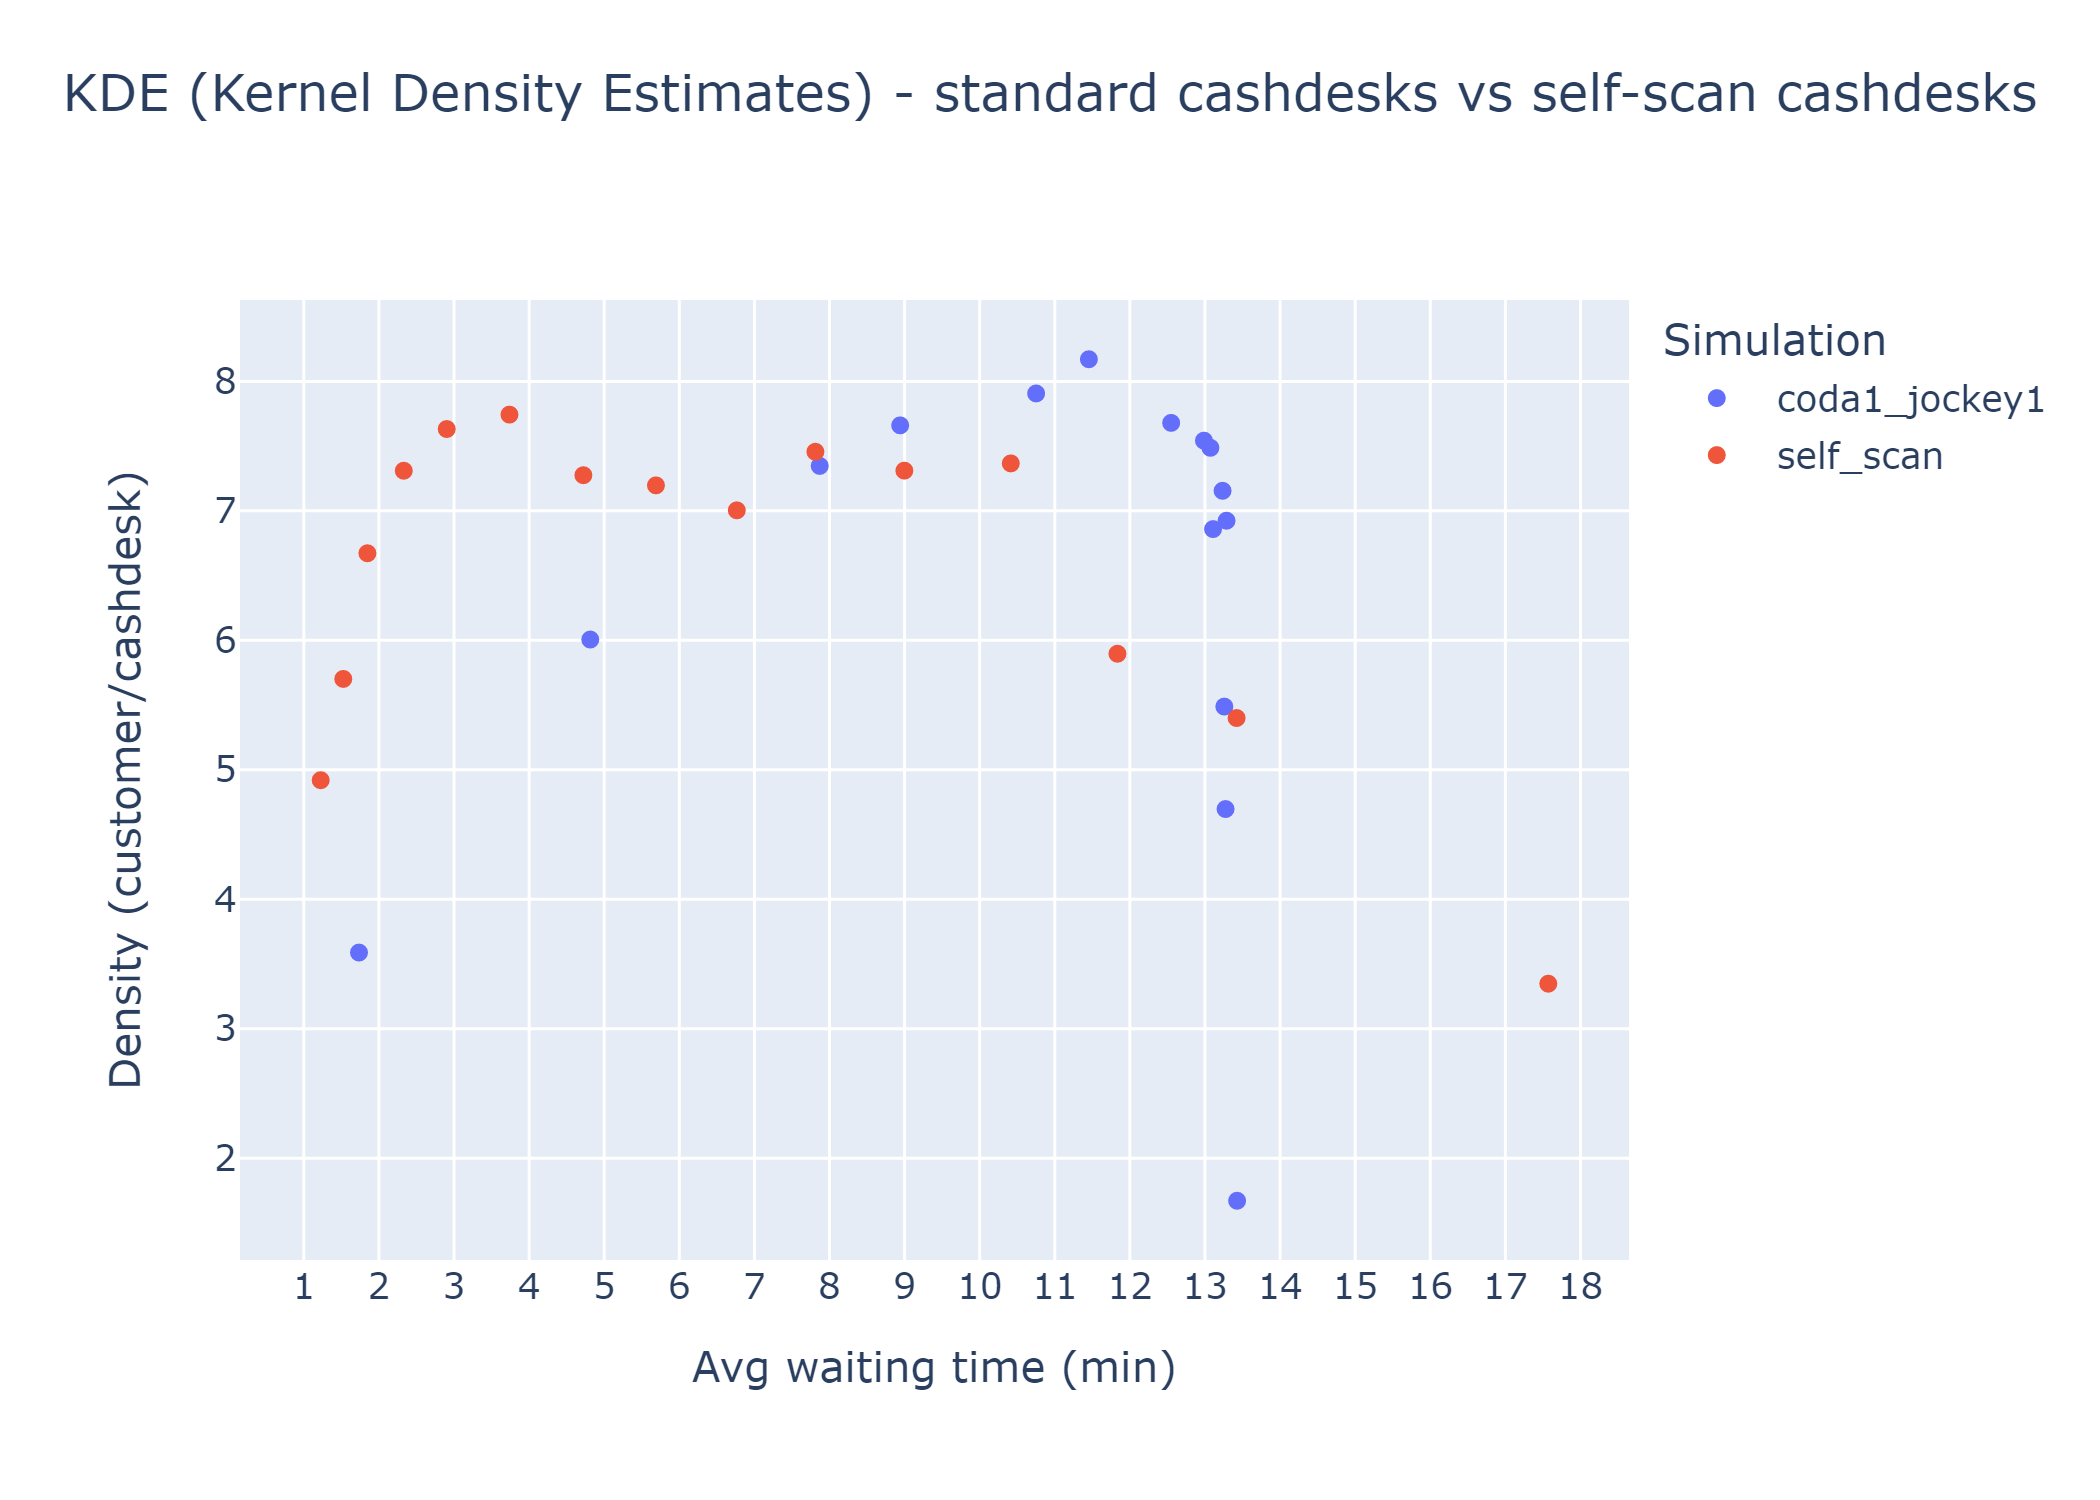
\includegraphics[width=12cm]{"images/results/kde_self_scan.png"}
	\label{fig:kde_self_scan}
	\caption{KDE - densità al variare del tempo medio d'attesa}
\end{figure}

L'immagine \ref{fig:kde_self_scan} mostra il grafico KDE della simulazione con sole casse self-scan messa a confronto con la simulazione con sole casse standard e jockey. Si nota che nella simulazione con casse standard c'è un momento di massima densità che viene gestito dal sistema portando a una diminuzione dei tempi medi d'attesa; nella simulazione con casse self-scan questa gestione della densità non avviene altrettanto bene, infatti dopo il punto critico di densità maggiore, questa diminuisce ma il tempo medio aumenta e questo è imputabile ancora una volta alle troppe persone che attendono di ricevere una rilettura della spesa.

\section{Simulazione non deterministica}

L'introduzione di parametri randomici rappresenta la nostra volontà di rendere più verosimile il modello e non un tentativo di miglioramento dei tempi medi d'attesa dei clienti. \\
Abbiamo voluto testare il modello completo, considerando 20 casse standard con code parallele, 6 casse self-service, 5 casse self-scan; la probabilità che un cliente sia self-scan (nel momento in cui entra nel negozio) è del $50\%$. Introduciamo anche l'errore di stima del basket-size da parte di un cliente: nel momento in cui un cliente deve calcolare il numero di elementi nel carrello di altri clienti commette un errore con 0.1 di deviazione standard. \\
Le simulazioni sono 8, combiniamo le strategie di scelta della coda (4) con quelle di jockey (2).

\begin{figure}[H]
	\centering
	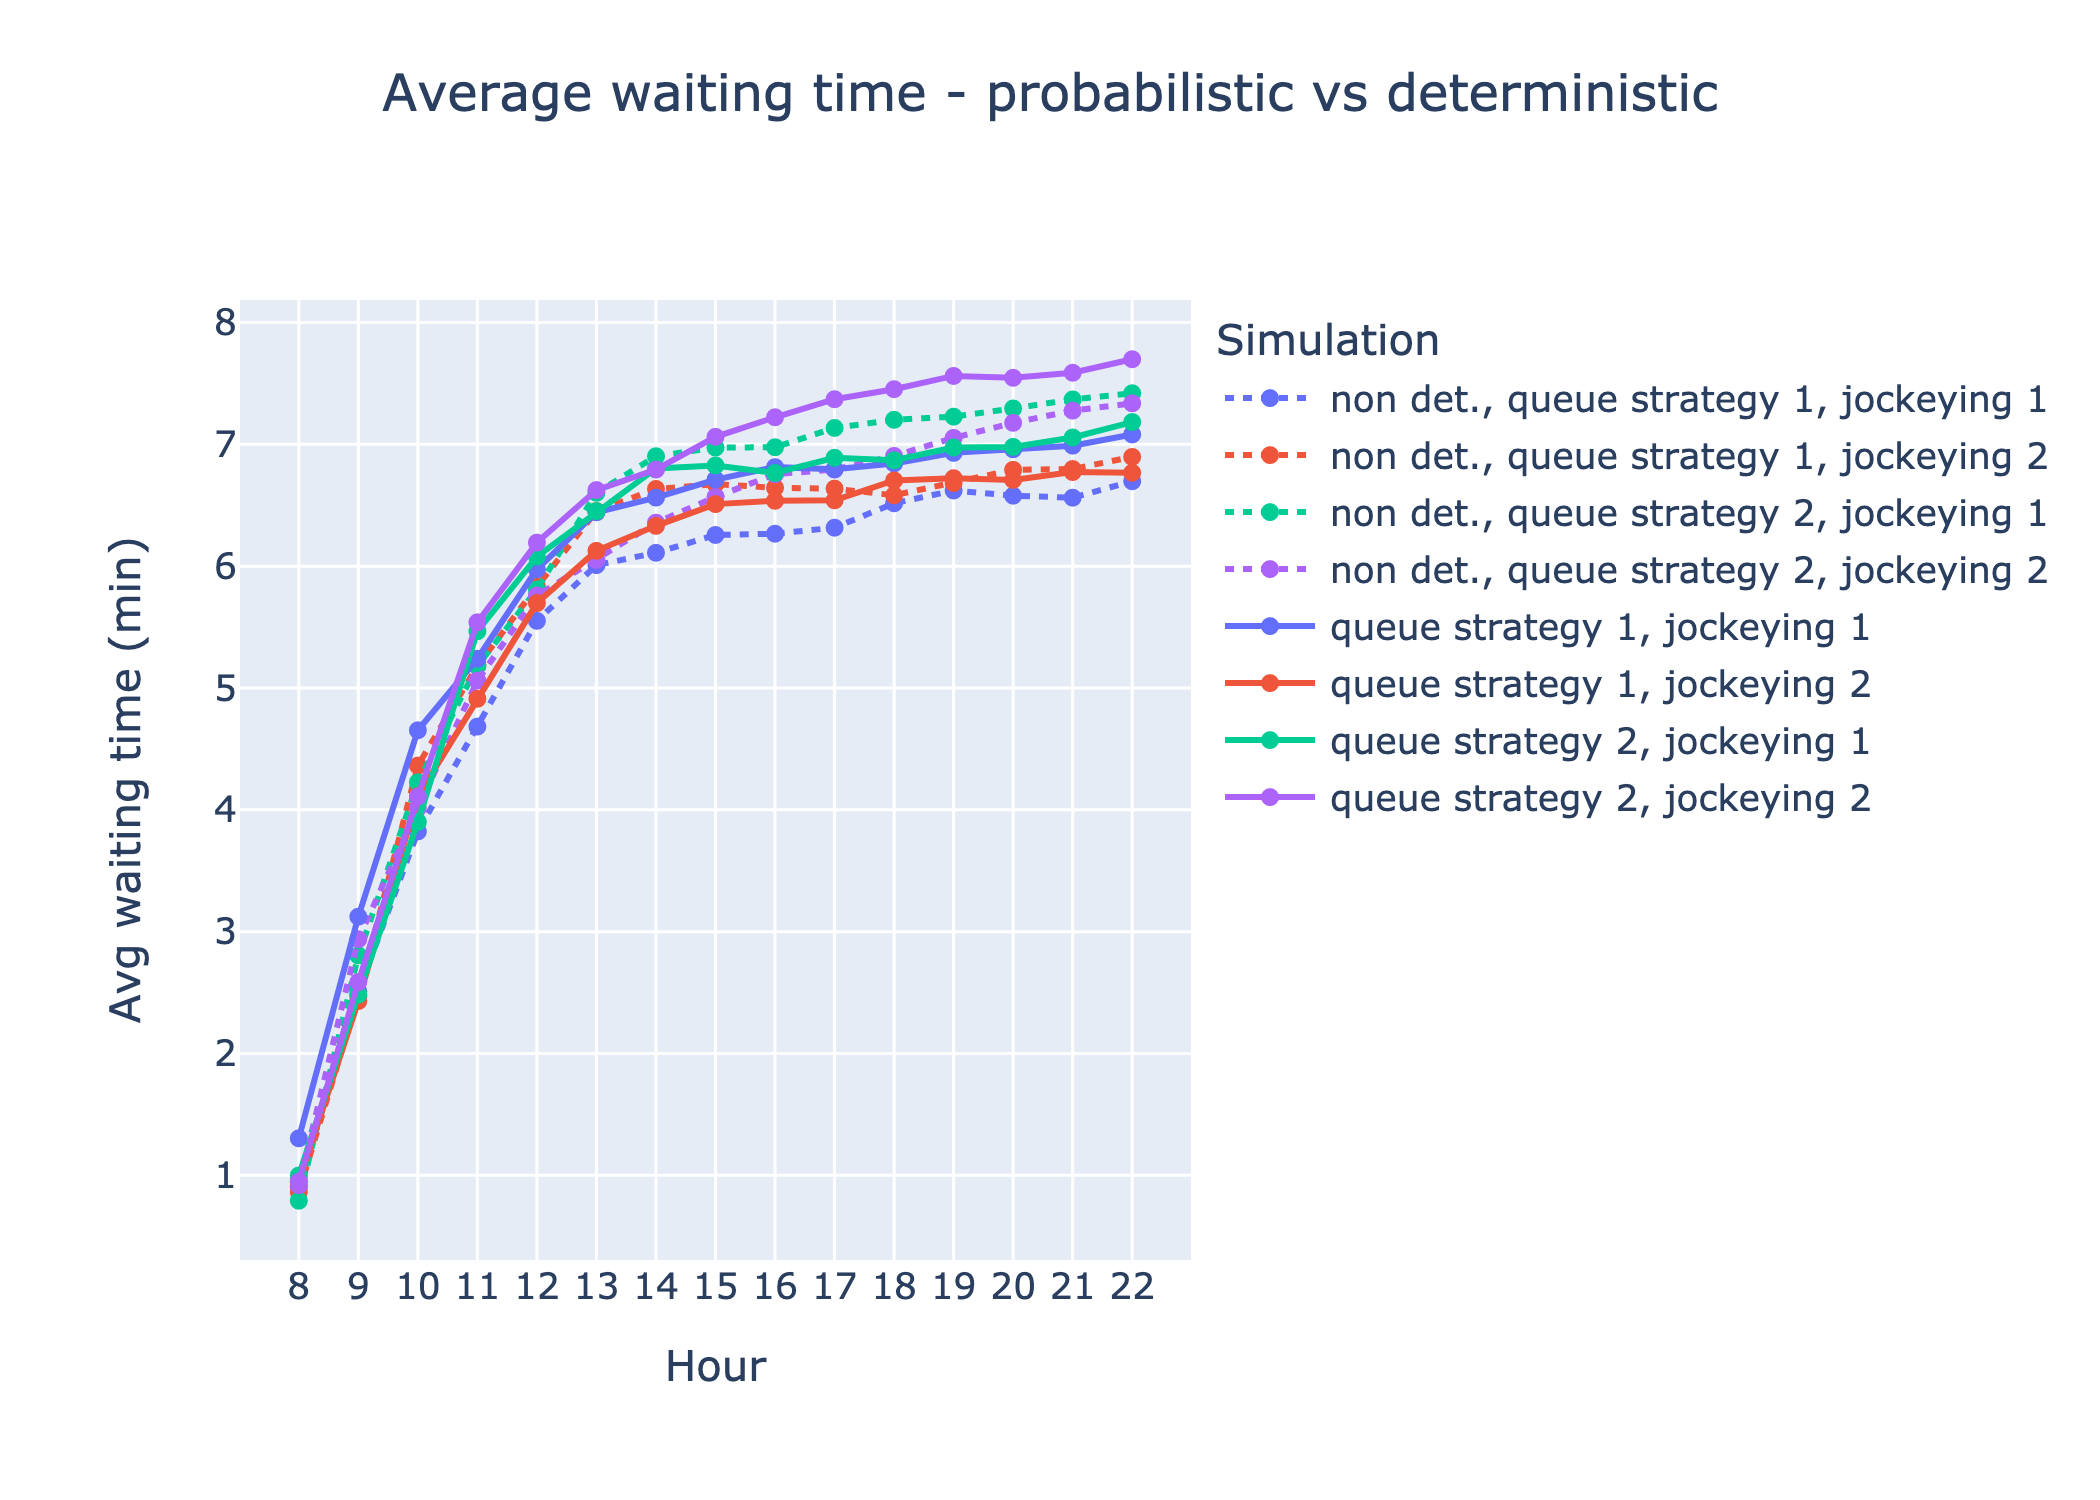
\includegraphics[width=12cm]{"images/results/avg_wt_prob.png"}
	\label{fig:avg_wt_prob}
	\caption{Tempo medio d'attesa al variare dell'ora}
\end{figure}

Notiamo dal grafico \ref{fig:avg_wt_prob} che il tempo medio d'attesa delle simulazioni con e senza elementi randomici (raggruppati a coppie per colore, una tratteggiata e una no) è assolutamente paragonabile e questo ci mostra che gli elementi che abbiamo aggiunto, giustificati dal buon senso, non scombinano totalmente il modello ma lo rendono semplicemente più imprevedibile, riuscendo a simulare più scenari possibili.

\vspace*{1\baselineskip}

Dopo aver condotto queste analisi possiamo concludere che il jockey da parte dei clienti porta a una diminuzione dei tempi d'attesa in coda e inoltre la configurazione delle casse a N-fork è in grado di gestire meglio il punto critico di densità di clienti rispetto alla configurazione a code parallele; nel prossimo capitolo verranno fatte le conclusioni e illustrati i possibili sviluppi futuri.
